\documentclass[a4paper,12pt,twoside]{../includes/ThesisStyle}
\usepackage[utf8]{inputenc}
\usepackage[T1]{fontenc}

\usepackage[left=1.5in,right=1.3in,top=1.1in,bottom=1.1in,includefoot,includehead,headheight=13.6pt]{geometry}\renewcommand{\baselinestretch}{1.05}


% =============================================================================
%\usepackage[sectionbib]{chapterbib}	% Cross-reference package (Natural BiB)
%\usepackage{bibunits}
%\usepackage{natbib}					% Put References at the end of each chapter
\usepackage{algorithm}
\usepackage{alltt}
\usepackage{amsfonts}
\usepackage{amsmath}
\usepackage{amssymb}
\usepackage{cite}
\usepackage{color}
\usepackage{enumerate}
\usepackage{booktabs} % used for \midrule
\usepackage{fancyhdr}					% Fancy Header and Footer
\usepackage{graphicx}
\usepackage{ifthen}
\usepackage{latexsym}
\usepackage{multirow}
\usepackage{rotating}					% Sideways of figures & tables
\usepackage{stmaryrd}
\usepackage{subfigure}
\usepackage{url}         
\usepackage{xspace}
\usepackage[normalem]{ulem} % for \sout
\usepackage{xcolor}
\usepackage{tablefootnote}
\usepackage{pifont}

% =============================================================================

% Table of contents for each chapter
\usepackage[nottoc, notlof, notlot]{tocbibind}
\usepackage{minitoc}
\setcounter{minitocdepth}{1}
\mtcindent=15pt

\setcounter{secnumdepth}{3}
\setcounter{tocdepth}{2}
  
% =============================================================================
% Fancy Header Style Options

\pagestyle{fancy}                       % Sets fancy header and footer
\fancyfoot{}                            % Delete current footer settings

%\renewcommand{\chaptermark}[1]{         % Lower Case Chapter marker style
%  \markboth{\chaptername\ \thechapter.\ #1}}{}} %

%\renewcommand{\sectionmark}[1]{         % Lower case Section marker style
%  \markright{\thesection.\ #1}}         %

\fancyhead[LE,RO]{\bfseries\thepage}    % Page number (boldface) in left on even
% pages and right on odd pages
\fancyhead[RE]{\bfseries\nouppercase{\leftmark}}      % Chapter in the right on even pages
\fancyhead[LO]{\bfseries\nouppercase{\rightmark}}     % Section in the left on odd pages

\let\headruleORIG\headrule
\renewcommand{\headrule}{\color{black} \headruleORIG}
\renewcommand{\headrulewidth}{1.0pt}
\usepackage{colortbl}
\arrayrulecolor{black}

\fancypagestyle{plain}{
  \fancyhead{}
  \fancyfoot{}
  \renewcommand{\headrulewidth}{0pt}
}


% =============================================================================
% Clear Header Style on the Last Empty Odd pages
\makeatletter

\def\cleardoublepage{\clearpage\if@twoside \ifodd\c@page\else%
  \hbox{}%
  \thispagestyle{empty}%              % Empty header styles
  \newpage%
  \if@twocolumn\hbox{}\newpage\fi\fi\fi}

\makeatother

\newenvironment{maxime}[1]
{
\vspace*{0cm}
\hfill
\begin{minipage}{0.5\textwidth}%
%\rule[0.5ex]{\textwidth}{0.1mm}\\%
\hrulefill $\:$ {\bf #1}\\
%\vspace*{-0.25cm}
\it 
}%
{%

\hrulefill
\vspace*{0.5cm}%
\end{minipage}
}

\let\minitocORIG\minitoc
\renewcommand{\minitoc}{\minitocORIG \vspace{1.5em}}


\renewcommand{\epsilon}{\varepsilon}

% centered page environment
\newenvironment{vcenterpage}
	{\newpage\vspace*{\fill}\thispagestyle{empty}\renewcommand{\headrulewidth}{0pt}}
	{\vspace*{\fill}}
	

%=============================================================================

\usepackage{needspace}
\newcommand{\needlines}[1]{\Needspace{#1\baselineskip}}

\usepackage{xcolor}
\definecolor{source}{gray}{0.95}
% source code formatting
\usepackage{listings}
    % global settings for source code listing package
\lstset{
    basicstyle=\ttfamily\small,
    showspaces=false,
    showstringspaces=false,
    captionpos=b, 
    columns=fullflexible}

\lstdefinelanguage{ST}{
    keywordsprefix=\#,
    morekeywords=[0]{true,false,nil},
    morekeywords=[1]{self,super,thisContext},
    morekeywords=[2]{ifTrue:,ifFalse:,whileTrue:,whileFalse:,and:,or:,xor:,not:,by:,timesRepeat:},
    sensitive=true,
    morecomment=[s]{"}{"},
    morestring=[d]',
    escapechar={!},
    alsoletter={., :, -, =, +, <},
    moredelim=**[is][\itshape]{/+}{+/},
    literate=
        {^}{{$\uparrow$}}1
        {:=}{{$\leftarrow$}}1
        {~}{{$\sim$}}1
        {-}{{\sf -\hspace{-0.13em}-}}1  % the goal is to make - the same width as +
        {+}{\raisebox{0.08ex}{+}}1		% and to raise + off the baseline to match V
        , % Don't forget the comma at the end!
    style=STStyle
}
\lstdefinestyle{STStyle}{
    tabsize=4,
    %frame=leftline,
    % frame=bl,
    %framerule=2pt,
    %rulecolor=\color{gray},
    % backgroundcolor=\color{white},
    %backgroundcolor=\usebeamercolor[bg]{listing},
    basicstyle=\ttfamily\small,
    keywordstyle=\bf\ttfamily,
    % stringstyle=\color{orange},
    stringstyle=\mdseries\slshape,
    commentstyle=\it\rmfamily\color{darkgray}, 
    commentstyle=\mdseries\slshape\color{gray},
    %commentstyle=\mdseries\slshape,
    emphstyle=\bf\ttfamily,
    escapeinside={!}{!},
	%backgroundcolor=\color{source},
    %emphstyle={[2]\color{red}},
    %emphstyle={[3]\color{blue}\bf},
    %emphstyle={[4]\color{blue}},
    keepspaces=true
} 

%\lstnewenvironment{javacode}  [1][]{\lstset{language=java,#1}\needlines{#2}}{} 
%\lstnewenvironment{pythoncode}[2][]{\lstset{language=python,#1}\needlines{#2}}{}
\lstnewenvironment{stcode}    [2][]{\lstset{language=ST,#1}\needlines{#2}}{}
\lstnewenvironment{ccode}     [2][]
    {\lstset{language=C,numbers=left,escapechar=\$,numberstyle=\tiny,#1}\needlines{#2}}{}

% ON: I tried to pass the line number options in as arg #1 but it does not work for me
% I also could net get the line numbers to consistently increase
\lstnewenvironment{numstcode} [2][]
    {\lstset{language=ST,numbers=left,numberstyle=\tiny,numbersep=2pt,#1}\needlines{#2}}{}
\lstnewenvironment{numstcodecont} [2][]
    {\lstset{language=ST,numbers=left,numberstyle=\tiny,numbersep=2pt,firstnumber=last#1}\needlines{#2}}{}

\newcommand{\lst}[1]{{\tt #1}}

% In-line code (literal)

% In-line code (latex enabled)
% Use this only in special situations where \ct does not work
% (within Section headings ...):
\newcommand{\lct}[1]{{\textsf{\textup{#1}}}}
% Code environments
\lstnewenvironment{code}{%
	\lstset{%
		% frame=lines,
		frame=single,
		framerule=0pt,
		mathescape=false
	}
}{}

%\renewcommand{\lstlistingname}{Code Example}

% =============================================================================
\newboolean{showcomments}
\setboolean{showcomments}{true}

\ifthenelse{\boolean{showcomments}} {
	\newcommand{\ugh}[1] {\textcolor{red}{\uwave{#1}}}	% please rephrase
	\newcommand{\ins}[1] {\textcolor{blue}{\uline{#1}}}	% please insert
	\newcommand{\del}[1] {\textcolor{red}{\sout{#1}}}	% please delete
	\newcommand{\chg}[2] {								% please change
		\textcolor{red}{\sout{#1}}{\ra}
		\textcolor{blue}{\uline{#2}}}
	\newcommand{\nbc}[3]{								% comment
		{\colorbox{#3}{\bfseries\sffamily\scriptsize\textcolor{white}{#1}}}
		{\textcolor{#3}{\sf\small$\blacktriangleright$\textit{#2}$\blacktriangleleft$}}}

}{
	\newcommand{\ugh}[1]{#1}							% please rephrase
	\newcommand{\ins}[1]{#1}							% please insert
	\newcommand{\del}[1]{}								% please delete
	\newcommand{\chg}[2]{#2}							% please change
	\newcommand{\nbc}[3]{}								% comment
}

% =============================================================================
\usepackage[pagebackref,hyperindex=true]{hyperref}


% Links in pdf
\usepackage{color}
\definecolor{linkcol}{rgb}{0.0, 0.0, 0.0} 
\definecolor{citecol}{rgb}{0.0, 0.0, 0.0} 

% Change this to change the informations included in the pdf file
% See hyperref documentation for information on those parameters
\hypersetup {
	bookmarksopen=true,
	pdftitle="Design and Use of Anatomical Atlases for Radiotherapy",
	pdfauthor="Olivier COMMOWICK", 
	pdfsubject="Creation of atlases and atlas based segmentation", %subject of the document
	%pdftoolbar=false, % toolbar hidden
	pdfmenubar=true, %menubar shown
	pdfhighlight=/O, %effect of clicking on a link
	colorlinks=true,
	pdfpagemode=UseNone,
	pdfpagelayout=SinglePage,
	pdffitwindow=true,
	linkcolor=linkcol,
	citecolor=citecol,
	urlcolor=linkcol
}

% =============================================================================
\newcommand{\figlabel}[1] {\label{fig:#1}}
\newcommand{\chaplabel}[1]{\label{chap:#1}}
\newcommand{\seclabel}[1] {\label{sec:#1}}
\newcommand{\tablabel}[1] {\label{tab:#1}}
\newcommand{\lstlabel}[1] {\label{lst:#1}}

\newcommand{\figref}[1] {Figure~\ref{fig:#1}}
\newcommand{\chapref}[1]{Chapter~\ref{sec:#1}}
\newcommand{\secref}[1] {Section~\ref{sec:#1}}
\newcommand{\tabref}[1] {Table~\ref{tab:#1}}
\newcommand{\lstref}[1] {Listing~\ref{tab:#1}}

\newcommand{\commented}[1]{}

\newcommand{\bs}    {\symbol{'134}} % backslash
\newcommand{\us}    {\symbol{'137}} % underscore
\newcommand{\ttt}[1]{\texttt{#1}}
\newcommand{\ie}    {\emph{i.e.},\xspace}
\newcommand{\eg}    {\emph{e.g.},\xspace}
\newcommand{\etal}  {\emph{et al.}\xspace}
\newcommand{\ns}    {\!\!\!\!} %big negative space
\newcommand{\cnull} {\textbackslash0\xspace}


\newcommand\fix[1]{\nb{FIX}{#1}}
\newcommand\todo[1]{\nb{TO DO}{#1}}
\newcommand\cb[1]{\nbc{CB}{#1}{purple}}
\newcommand\sd[1]{\nbc{SD}{#1}{orange}}
\newcommand\is[1]{\nbc{IS}{#1}{gray}}
\newcommand\gc[1]{\nbc{GC}{#1}{olive}}
\newcommand\ct[1]{\nbc{CT}{#1}{teal}}
\newcommand\md[1]{\nbc{MD}{#1}{blue}}
\newcommand\dc[1]{\nbc{DC}{#1}{green}}

% =============================================================================
\newcommand{\NBFFI}  {Native\-Boost-FFI\xspace}
\newcommand{\NB}  {Native\-Boost\xspace}
\newcommand{\B}   {Benzo\xspace}
\newcommand{\ST}  {Small\-talk\xspace}
\newcommand{\PH}  {Pharo\xspace}
\graphicspath{{.}{../figures/}}

\begin{document}
% ==========================================================================
\chapter{Validation: \FFI}
\chaplabel{ffi}
\minitoc
% ===========================================================================
\introduction
% ===========================================================================

In the previous \chapref{benzo} we presented \B, a framework that spans over several abstraction layers to enable low-level programming.
\B is the generic backend for a variety of applications we outlined in the previous chapter: a Foreign-Function-Interface \FFI, a prototype for dynamic primitives and a prototype for a language-side \JIT compiler.
In this chapter we present the most mature \B application, the \FFI which is success	fully used in production in \PH 2.0 an newer.

\FFIs are a prerequisite for close system integration of a high-level language.
With \FFIs the high-level environment interacts with low-level functions allowing for a unique combination of features.
This need to interconnect high-level (Objects) and low-level (C functions) has a strong impact on the implementation of a FFI: it has to be flexible and fast at the same time.

We propose \NB a language-side approach to \FFIs that only requires minimal changes to the VM.
\NB directly creates specific native code at language-side and thus combines the flexibility of a language-side library with the performance of a native plugin.
\todo{probably write a bit more...}

% ===========================================================================
\newpage
\section{Background}
\seclabel{ffi-background}
% ===========================================================================

Currently, more and more code is produced and available through reusable libraries such as \urlfootnote{OpenGL}{http://www.opengl.org/} or \urlfootnote{Cairo}{http://cairographics.org/}.
While working on your own projects using dynamic languages, it is crucial to be able to use such existing libraries with little effort.
Multiple solutions exist to achieve access to an external library from dynamic languages that are executed on the top of a virtual machine (\VM) such as \urlfootnote{\PH}{http://pharo.org/}, \urlfootnote{\Lua}{http://lua.org/} or \urlfootnote{\Python}{http://python.org/}.
\figref{benzo-extensionComparison} depicts four possibilities of dealing with new or external libraries in a high-level language.

\paragraph{Language-side Library}
One solution is to re-implement a library completely at language-side (cf. \figref{benzo-extensionComparison}.a).
Even though this is the most flexible solution, this is often not an option, neither from the technical point of view (performance penalty), nor from the economic point of view (development time and costs).

\paragraph{\VM Extension}
The second one (\figref{benzo-extensionComparison}.b) is to do a \emph{\VM extension} providing new primitives that the high-level language uses to access the native external library.
This solution is generally efficient since the external library may be statically compiled within the \VM.
However a tight integration into the \VM also means more dependencies and a different development environment than the final product at language-side.

\paragraph{\VM Plugin}
The third solution (\figref{benzo-extensionComparison}.c) is similar to the previous one but the extension is factored out of the \VM as a \emph{plugin}.
This solution implies again a lot of low-level development at \VM-level that must be done for each external library we want to use.
Additionally we have to adapt the plugin for all platforms on which the \VM is supposed to run on.

\paragraph{\FFI}
A higher-level solution is to define \emph{Foreign Function Interfaces} (\FFIs) (cf. \figref{benzo-extensionComparison}.d).
The main advantage of this approach is that once a \VM is \FFI-enabled, only a language extension (no \VM-level code) is needed to provide access to new native libraries.
From the portability point of view, only the generic \FFI \VM-plugin has to be implemented on all platforms.

Implementing an \FFI library is a challenging task because of its antagonist goals:
\begin{itemize}
    \item it must be flexible enough to easily bind to external libraries and also express complex foreign calls regarding the memory management or the type conversions (marshalling);
    \item it must be well integrated with the language (objects, reflection, garbage collector);
    \item it must be efficient.
\end{itemize}
%
Existing \FFI libraries of dynamic languages all have different designs and implementations because of the trade-offs they made regarding these goals and challenges.
Typical choices are resorting purely to the \VM-level and thus sacrificing flexibility.
The inverse of this approach exists as well: \FFIs can be implemented almost completely at language-side but at a significant performance loss.
Both these pitfalls are presented in more detail in \secref{ffi-evaluation}.

This chapter presents \urlfootnote{\NBFFI}{http://code.google.com/p/nativeboost/} an \FFI library at language-side for \PH that supports callouts and callbacks, which we present in \secref{ffi-nutshell}.
There are at least two other existing \FFI libraries in \PH worth mentioning: C-\FFI and \Alien.
Nevertheless, they both present shortcomings.
C-\FFI is fast because it is mostly implemented at \VM-level, however it is limited when it comes to do complex calls that involve non-primitive types or when we want to define new data types.
On the opposite, \Alien \FFI is flexible enough to define any kind of data conversion or new types directly at language-side but it is slower than C-\FFI because it is mostly implemented at language-side.
In essence, \NBFFI combines the flexibility and extensibility of \Alien that uses language-side definition for marshalling and the speed of C-\FFI which is implemented at \VM-level.
The main contributions of \NBFFI are:

\begin{description}
	\item[Extensibility.] \NBFFI relies on as few \VM primitives as possible (5 primitives), essentially to call native code. 
	Therefore, most of the implementation resides at language-side, even low-level mechanisms.
	That makes \NBFFI easily extensible because its implementation can be changed at any time, without needing to update the runtime (\VM).
	It also presents a noticeable philosophical shift, how we want to extend our language in future.
	A traditional approach is to implement most low-level features at \VM-side and provide interfaces to the language-side.
	But that comes at cost of less flexibility and longer development and release cycles.
	On the opposite, we argue that extending language features, even low-level ones, should be done at language-side instead.
	This results in higher flexibility and without incurring high runtime costs which usually happen when using high-level languages such as \PH.
	\item[Language-side extension.] Accessing a new external library using \NBFFI involves a reduced amount of work since it is only a matter of writing a language-side extension.
	\item[Performance.] Despite the fact it is implemented mostly at language-side, \NBFFI achieves superior performance compared to other \FFI implementations running \PH.
    This is essentially because it uses automatic and transparent native code generation at language-side for marshalling.
\end{description}


% ===========================================================================
\section{\NBFFI: an Introduction}
\seclabel{ffi-nutshell}
% ===========================================================================

This section gives an overview of the code that should be written at language-side
to enable interactions with external libraries.


% ---------------------------------------------------------------------------
\subsection{Simple Callout}
% ---------------------------------------------------------------------------

\lstref{ffi-clock} shows the code of a regular \PH method named \ttt{ticksSinceStart} that defines a callout to the \ttt{clock} function of the \ttt{libc}.
\NB imposes no constraint on the class in which such a binding should be defined.
However, this method must be annotated with a specific pragma (such as \ttt{<primitive:module:>}) which specifies that a native call should be performed using the \NB plugin.

\begin{stcode}[
	label={lst:ffi-clock},
	caption={\NBFFI example of callout declaration to the \ttt{clock} function of the \ttt{libc}}]{0}
ticksSinceStart
	<primitive: #primitiveNativeCall
	 module: #NativeBoostPlugin>
	^ self
		nbCall: #(uint clock ())
		module: NativeBoost CLibrary
\end{stcode}

\noindent The external function call is then described using the \ttt{nbCall:module:} message.
The first parameter (\ttt{\#nbCall:}) is an array that describes the signature of C function to callout.
Basically, this array contains the description of a C function prototype, which is very close to normal C syntax.
The return type is first described (\ttt{uint} in this example\footnote{The return type of the \ttt{clock} function is \ttt{clock\_t}, but we deliberately used \ttt{uint} in this first example for the sake of simplicity even if it is possible to define a constant type in \NB.}), then the name of the function (\ttt{clock}) and finally the list of parameters (an empty array in this example since \ttt{clock} does not have any).
The second argument, \ttt{\#module:} is the module name, its full path or its handle if already loaded, where to look up the given function.
This example uses a convenience method of \NB named \ttt{CLibrary} to obtain a handle to the standard C library.

% ---------------------------------------------------------------------------
\subsection{Callout with Parameters}
\seclabel{ffi-callout-parameters}
% ---------------------------------------------------------------------------

\figref{ffi-nativeBoostSyntax} presents the general syntax of \NBFFI through an example of a callout to the \ttt{abs} function of the \ttt{libc}.
The \ttt{abs:} method has one argument named \ttt{anInteger} (cf. \ding{182}).
This method uses the pragma \ttt{<primitive:module:error:>} which indicates that the \ttt{\#primitiveNativeCall} of the \ttt{\#NativeBoostPlugin} should be called when this method is executed (cf. \ding{183}).
An \ttt{errorCode} is returned by this primitive if it fails and the regular \PH code below is executed (cf. \ding{184}).
The main difference with the previous example is that the \ttt{abs} function takes one integer parameter.
In this example, the array \ttt{\#(uint abs(int anInteger))} passed as argument to \ttt{\#nbCall:} contains two important information (cf. \ding{185}).
First, the types annotations such as the return type (\ttt{uint} in both examples) and arguments type (\ttt{int} in this example).
These types annotations are then used by \NBFFI to automatically do the marshalling between C and \PH values as illustrated by the next example.
Second, the values to be passed when calling out.
In this example, \ttt{anInteger} refers to the argument of the \ttt{abs} method, meaning that the value of this variable should be passed to the \ttt{abs} C function.
Finally, this \ttt{abs} function is looked up in the \ttt{libc} whose an handle is passed in the \ttt{module:} parameter (cf. \ding{186}).

\begin{figure}[H]
	\centering
	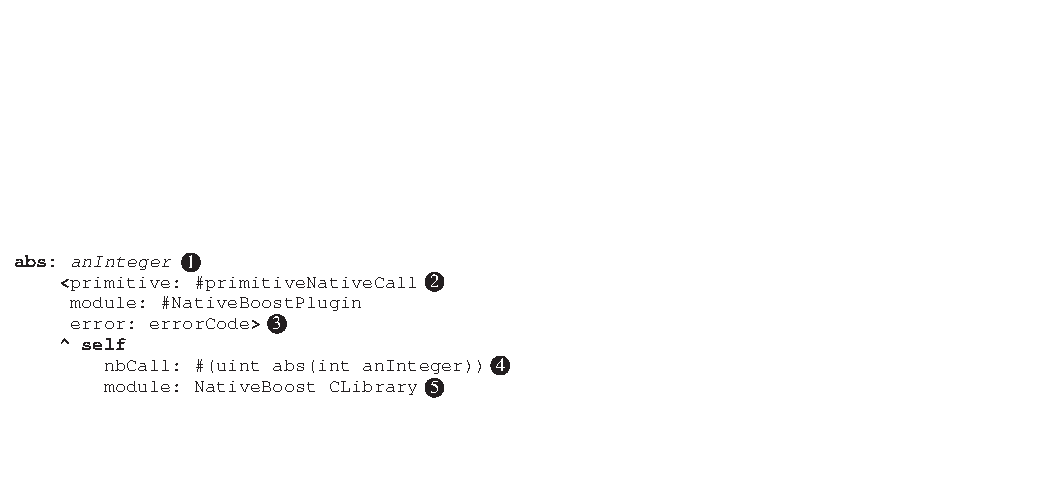
\includegraphics[scale=1.2]{nativeBoostSyntax}
	\caption[\NB Basic Method]{Example of the general \NBFFI callout syntax}
	\figlabel{ffi-nativeBoostSyntax}
\end{figure}

% ---------------------------------------------------------------------------
\subsection{Automatic Marshalling of Known Types}
% ---------------------------------------------------------------------------

\lstref{ffi-getenv} shows a callout declaration to the \ttt{getenv} function that takes one parameter.
%
\begin{stcode}[
	label={lst:ffi-getenv},
	caption={Example of callout to \ttt{getenv}}]{0}
getenv: name
	<primitive: #primitiveNativeCall
	 module: #NativeBoostPlugin>

	^ self
		nbCall: #(String getenv(String name)
		module: NativeBoost CLibrary
\end{stcode}
%
In this example, the \NB type specified for the parameter is \ttt{String} instead of \ttt{char*} as specified by the standard \ttt{libc} documentation.
This is on purpose because strings in C are sequences of characters (\ttt{char*}) but they must be terminated with the special character: \cnull.
Specifying \ttt{String} in the \ttt{\#nbCall:} array will make \NB to automatically do the arguments conversion from \PH strings to C strings (\cnull terminated \ttt{char*}).
It means that the string passed will be put in an external C \ttt{char} array and a \cnull character will be added to it at the end.
This array will be automatically released after the call returned.
This is an example of automatic memory management of \NB that can also be controlled if needed.
Obviously, the opposite conversion happens for the returned value and the method returns a \PH string.
This example shows that \NBFFI accepts literals, local and instance variable names in callout declarations and it uses their type annotation to achieve the appropriate data conversion.
\tabref{ffi-nbPrimitiveTypes} shows the default and automatic data conversions achieved by \NBFFI.

\begin{table}[hbt]
    \centering
    \begin{tabular}{rll}
        Primitive Type       & \PH Type \\\midrule
        \ttt{uint}   & \ttt{Integer} \\
        \ttt{int}    & \ttt{Integer} \\
        \ttt{String} & \ttt{ByteString} \\
        \ttt{bool}   & \ttt{Boolean} \\
        \ttt{float}  & \ttt{Float} \\
        \ttt{char}   & \ttt{Character} \\
        \ttt{oop}    & \ttt{Object}
    \end{tabular}
    \caption[\NB Primitive Types]{Default \NBFFI mappings between C/primitive types and high-level types. Note that \ttt{oop} is not a real primitive type as no marshalling is applied and the raw pointer is directly exposed to \PH.}
    \tablabel{ffi-nbPrimitiveTypes}
\end{table}

\noindent \lstref{ffi-setenv} shows another example to callout the \ttt{setenv} function.
The return value will be converted to a \PH \ttt{Boolean}.
The two first parameters are specified as \ttt{String} and will be automatically transformed in \ttt{char*} with an ending \cnull character.
The last parameter is \ttt{1}, a \PH literal value without any type specification and \NB translates it as an \ttt{int} by default.

\begin{stcode}[
	label={lst:ffi-setenv},
	caption={Example of callout to \ttt{setenv}}]{0}
setenv: name value: value
	<primitive: #primitiveNativeCall
	 module: #NativeBoostPlugin>

	^ self
		nbCall: #(Boolean setenv(String name,
								 String value,
								 1)
		module: NativeBoost CLibrary
\end{stcode}

\noindent Another interesting example of automatic marshalling is to define the \ttt{abs} method (cf. \figref{ffi-nativeBoostSyntax}) in the \ttt{SmallInteger} class and passing \ttt{self} as argument in the callout.
In such case, \NB automatically converts \ttt{self} (which is a \ttt{SmallInteger}) into an \ttt{int}.
This list of mapping is not exhaustive and \NB also supports the definition of new data types and new conversions into more complex C types such as structures (cf. \secref{ffi-internals}).

% memory alloc & structs
\begin{table}[h]
	\begin{adjustwidth}{-2.0in}{-2.0in}
	\centering
    \begin{tabular}{lllll}
                    &  Memory 	    & Address  & Marshalling         & Constraint  \\\midrule
C-managed struct 	&  C heap  	    & fixed    & passed by reference & must be freed \\
\multirow{2}{*}{\PH-managed struct}  & \multirow{2}{*}{Object memory} & \multirow{2}{*}{variable} & passed by reference & may move \\
& & & passed by copy & costly\\
    \end{tabular}
    \end{adjustwidth}
    \caption{Choice of wrapping structures in \NB}
    \tablabel{ffi-wrappingstruct}
\end{table}


% ---------------------------------------------------------------------------
\subsection{Supporting new types}
\seclabel{ffi-newtypes}
% ---------------------------------------------------------------------------

The strength of language-side \FFIs appears when it comes to do callouts with new data types involved.
\NBFFI supports different possibilities to interact with new types.

\paragraph{Declaring structures}
For example, the \urlfootnote{Cairo library}{http://cairographics.org/} provides complex structures such as \ttt{cairo\_surface\_t} and functions to manipulate this data type. % which makes field access useless.
\lstref{ffi-AthensCairoSurface} shows how to write a regular \PH class to wrap a C structure.
\NB only requires a class-side method named \ttt{asNBExternalType:} that describes how to marshall this type back and forth from native code.
In this example, we use existing marshalling mechanism defined in \ttt{NBExternalObjectType} that just copies the structure's pointer and stores it in an instance variable named \ttt{handle}.

\begin{stcode}[
	label={lst:ffi-AthensCairoSurface},
	caption={Example of C structure wrapping in \NB}]{0}
AthensSurface subclass: #AthensCairoSurface
	instanceVariableNames: 'handle'.

AthensCairoSurface class>>asNBExternalType: gen
	"handle iv holds my address (cairo_surface_t)"
	^ NBExternalObjectType objectClass: self
\end{stcode}

\paragraph{Callout with structures}
\lstref{ffi-calloutOpaqueStruct} shows a callout definition to the \ttt{cai\-ro\_image\_surface\_create} function that returns a \ttt{cairo\_surface\_t*} data type.
In this code example, the return type is \ttt{AthensCairoSurface} directly (not a pointer).
When returning from this callout, \NB creates an instance of \ttt{AthensCairoSurface} and the marshalling mechanism  stores the returned address in the \ttt{handle} instance variable of this object.

\begin{stcode}[
	label={lst:ffi-calloutOpaqueStruct},
	caption={Example of returning a structure by reference}]{0}
primImage: aFormat width: aWidth height: aHeight
	<primitive: #primitiveNativeCall
	 module: #Benzo
     error: errorCode>

	^self nbCall: #(AthensCairoSurface
		cairo_image_surface_create (int aFormat,
									int aWidth,
									int aHeight) )
\end{stcode}

\noindent Conversely, passing an \ttt{AthensCairoSurface} object as a parameter in a callout makes its pointer stored in its \ttt{handle} iv (cf. \lstref{ffi-calloutOpaqueStructParameter}) to be passed.
Since the parameter type is \ttt{AthensCairoSurface} in the callout definition, \NB also ensures that the passed object is really an instance of this class.
If it is not, the callout fails before executing the external function because passing it an address on a non-expected data could lead to unpredicted behavior.

\begin{stcode}[
	label={lst:ffi-calloutOpaqueStructParameter},
	caption={Example of passing a structure by reference}]{0}
primCreate: cairoSurface
	<primitive: #primitiveNativeCall module: #Benzo >

	^self nbCall: #(
        AthensCairoCanvas cairo_create (
                  AthensCairoSurface cairoSurface))
\end{stcode}


\paragraph{Accessing structure fields}
In \NB, one can directly access the fields of a structure if needed, even if it is not a good practice from the data encapsulation point of view.
Nevertheless, it may be mandatory to interact with some native libraries that do not provide all the necessary functions to manipulate the structure.
\lstref{ffi-cairo_c_definition} shows an example of a C struct type definition for \ttt{cairo\_matrix\_t}.

\begin{numstcode}[
	label={lst:ffi-cairo_c_definition},
	caption={Example external type to convert back and forth with the Cairo library}]{0}
typedef struct {
    double xx; double yx;
    double xy; double yy;
    double x0; double y0;
} cairo_matrix_t;
\end{numstcode}

\noindent \lstref{ffi-AthensCairoMatrix} shows that the \ttt{NBExternalStructure} of \NBFFI can be subclassed to define new types such as \ttt{AthensCairoMatrix}.
The description of the fields (types and names) of this structure is provided by the \ttt{fieldsDesc} method on the class side.
Given this description, \NB lazily generates field accessors on the instance side using the field names.

\begin{numstcode}[
	label={lst:ffi-AthensCairoMatrix},
	caption={Example of \NBFFI definition of an \ttt{ExternalStructure}}]{0}
NBExternalStructure
    variableByteSubclass: #AthensCairoMatrix.

AthensCairoMatrix class>>fieldsDesc
	^ #(  double sx; double shx;
		  double shy; double sy;
		  double x; double y;  )
\end{numstcode}

\noindent \lstref{ffi-cairoCallouts} shows a callout definition to the
 \ttt{cairo\_matrix\_multiply} function passing \ttt{self} as argument with the type \ttt{AthensCairoMatrix*}.
\NB handles the marshalling of this object to a struct as defined in the \ttt{fieldsDesc}.
% The interesting point is that the called function \ttt{cairo\_matrix\_multiply} stores its result in the first argument i.e. the receiver object.

\begin{numstcode}[
	label={lst:ffi-cairoCallouts},
	caption={Example of callouts using \ttt{cairo\_matrix\_t}}]{0}
AthensCairoMatrix>>primMultiplyBy: m
	<primitive: #primitiveNativeCall
	 module: #Benzo
     error: errorCode>

"C signature"
"void cairo_matrix_multiply (
                     cairo_matrix_t *result,
                     const cairo_matrix_t *a,
                     const cairo_matrix_t *b );"
	^self nbCall: #(void   cairo_matrix_multiply
		(AthensCairoMatrix * self,
		AthensCairoMatrix * m ,
		AthensCairoMatrix * self ) )
\end{numstcode}


\paragraph{Memory management of structures}
\tabref{ffi-wrappingstruct} shows a comparison between C-managed and \PH-managed structures.
The first ones are allocated in the C heap.
Their addresses are fixed and they are passed by reference during a callout.
But the programmer must free them by hand when they are not needed.
The second ones are allocated in the \PH object-memory.
Their addresses are variable since their enclosing object may be moved by the garbage collector.
They can either passed by copy which is costly or by reference.
Passing a reference may lead to problems is the C function stores the address and try to access it later on since the address may changed.


% ---------------------------------------------------------------------------
\subsection{Callbacks}
% ---------------------------------------------------------------------------

\NB supports callbacks from native code.
This means it is possible for a C-function to call back into the \PH runtime and activate code.
We will use the simple \ttt{qsort} C-function to illustrate this use-case.
\ttt{qsort} sorts a given array according to the results of a compare function.
Instead of using a C-function to compare the elements we will use a callback to invoke a \PH block which will compare the two arguments.
%
\begin{stcode}[
	label={lst:ffi-calloutWithCallback},
	caption={Example of callout passing a callback for \ttt{qsort}}]{0}
bytes := #[ 120 12 1 15 ].
callback := QSortCallback on: [ :a :b |
				(a byteAt: 0) - (b byteAt: 0) ].

self ffiQSort: bytes
	 length: bytes size
	 compareWith: callback
\end{stcode}
%
Code \lstref{ffi-calloutWithCallback} shows the primary \PH method for invoking \ttt{qsort} with a \ttt{QSortCallback} instance for the compare function.
In this example \ttt{qsort} will invoke run the \PH code inside the callback block to compare the elements in the \ttt{bytes} array.

To define a callback in \NB we have to create a specific subclasses for each callback with different argument types.
%
\begin{stcode}[
	label={lst:ffi-callbackDefinition},
	caption={Example of callback definition}]{0}

NBFFICallback
    subclass: #QSortCallback.

NBFFICallback class>>signature
	^#(int (NBExternalAddress a, NBExternalAddress b))
\end{stcode}
%
Code \lstref{ffi-callbackDefinition} shows \ttt{QSortCallback} which takes two generic external addresses as arguments.
These are the argument types that are being passed to the sort block in Example \lstref{ffi-calloutWithCallback}.
%
\begin{stcode}[
	label={lst:ffi-qsort},
	caption={Example of callout passing a callback}]{0}
ffiQSort: base len: size compare: qsortCallback
	<primitive: #primitiveNativeCall module: #Benzo>

	"C qsort signature"
	"void qsort(
		void *base,
		size_t nel,
		size_t width,
		int (*compar)(const void *, const void *));"

	^ self
		options: #( optMayGC )
		nbCall: #(void qsort (
					NBExternalAddress array,
					ulong size,
					1, "sizeof an element"
					QSortCallback qsortCallback))
		module: NativeBoost CLibrary
\end{stcode}
%
The last missing piece in this example is the callout definition shown in Code \lstref{ffi-qsort}.
The \NB callout specifies the callback arguments by using \ttt{QSortCallback}.

%\begin{enumerate}
%	\item Define a callback by subclassing NBCallback and overriding \ttt{\#fnSpec} method that defines de C signature of the callback
	% Redefining callback signature.
% A callback uses a lazy-initialization scheme to generate a common marshalling code which will be used by all instances of specific callback class.
% So, changing a callback signature (by changing its #fnSpec method) will not have an immediate effect, if you already created at least a single instance of it.
% To make changes take effect, you must restart an image.

%	\item Define a callout as previously but passing a callback as argument using its class name as argument type.

% !!Note!! A special care must be taken for all functions which may make callbacks!
% In the above qsort() example, you can see an additional option for external call - #optMayGC, which tells a code generator to call an external function via call gate (a special stub which handling a code relocation caused by \GC). Thats it, for any external functions, which may call the callback you must pass this option.
% Rationale: since most of external functions don't make any callbacks (and so has no chance to trigger \GC), using this option by default will be an overkill, which will just spend extra CPU cycles for nothing.
% However, if you omit this option when calling the function(s) which may call back, expect a hard crash(es) to happen.

%	\item instantiate the callback giving it a block.
	% To use callbacks, you must instantiate it first by passing block as an argument:
% mycallback := MyCallback on: someBlock.

% The block is the closure which will be evaluated when callback function get called, so the block must take same number of arguments as specified in #fnSpec method, and its evaluation result must yield a value which can be converted back C type value, which you speficied as a return type of callback function.
% For example, if callback signature is 'int (int foo , float bar )' , we can create a callback with following block closure:

% mycallback := MyCallback on: [:foo :bar |  (foo + bar ) asInteger ].


\paragraph{Callback lifetime}
Each time a new callback is instantiated it reserves a small amount of external memory which is freed once the callback is no longer used.
This is done automatically using object finalization hooks..


% ===========================================================================
\subsection{Overview of \NBFFI Internals}
% - explain how code is generated in simple steps, not going into details

This section provides an overview of the internal machinery of \NBFFI though it is not mandatory to know it in order to use it as demonstrated by previous examples.

\paragraph{General Architecture}
\figref{ffi-nbArchitecture} describes the general architecture of \NB.
Most code resides at language-side, nevertheless some generic extensions (primitives) to the \VM are necessary to activate native code.
At language-side, callouts are declared with \NBFFI which processes them and dynamically generates x86 native code using the \ttt{AsmJit} library.
This native code is responsible of the marshalling and calling the external function.
\NB then uses a primitive to activate this native code.

\begin{figure}[ht]
	\centering
	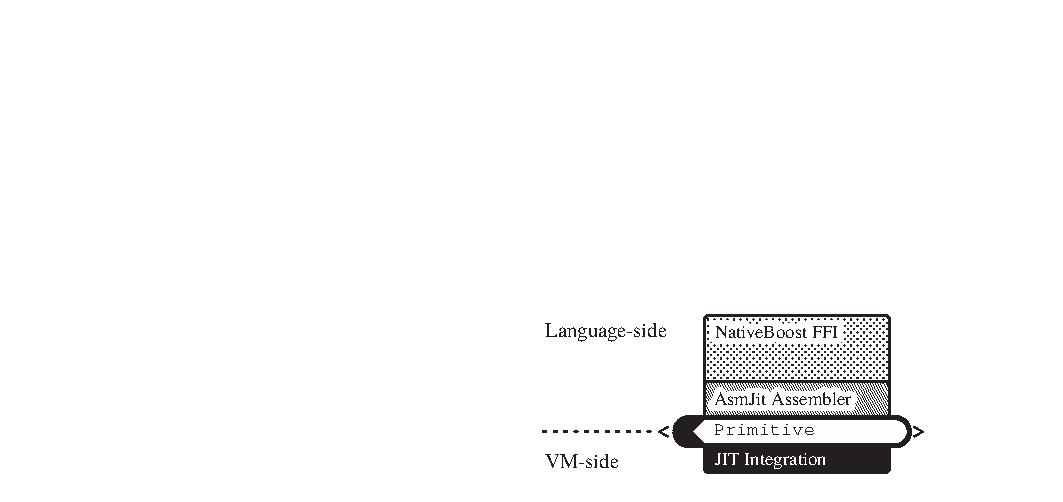
\includegraphics[scale=1.1]{nbArchitecture}
	\caption[\NB Components Layering]{\NB main components that major part of the code resides at language-side.}
	\figlabel{ffi-nbArchitecture}
\end{figure}

\paragraph{Callout propagation}
\figref{ffi-ffi} shows a comparison of the resolution of a \FFI call both in \NBFFI and a plugin-based \FFI.
At step 1, a \FFI call is emitted.
The \NBFFI call is mostly processed at language-side and it is only during step 4 that a primitive is called and the \VM effectively does the external call by executing the native code.
On the opposite, a plugin-based \FFI call already crossed the low-level frontier in step 2 resulting that part of the type conversion process (marshalling) is already done in the \VM code.
In \NBFFI, doing most of the \FFI call processing at language-side makes easier to keep control, redefine or adapt it if needed.

\begin{figure*}[h]
	\begin{adjustwidth}{-2.0in}{-2.0in}
		\centering
		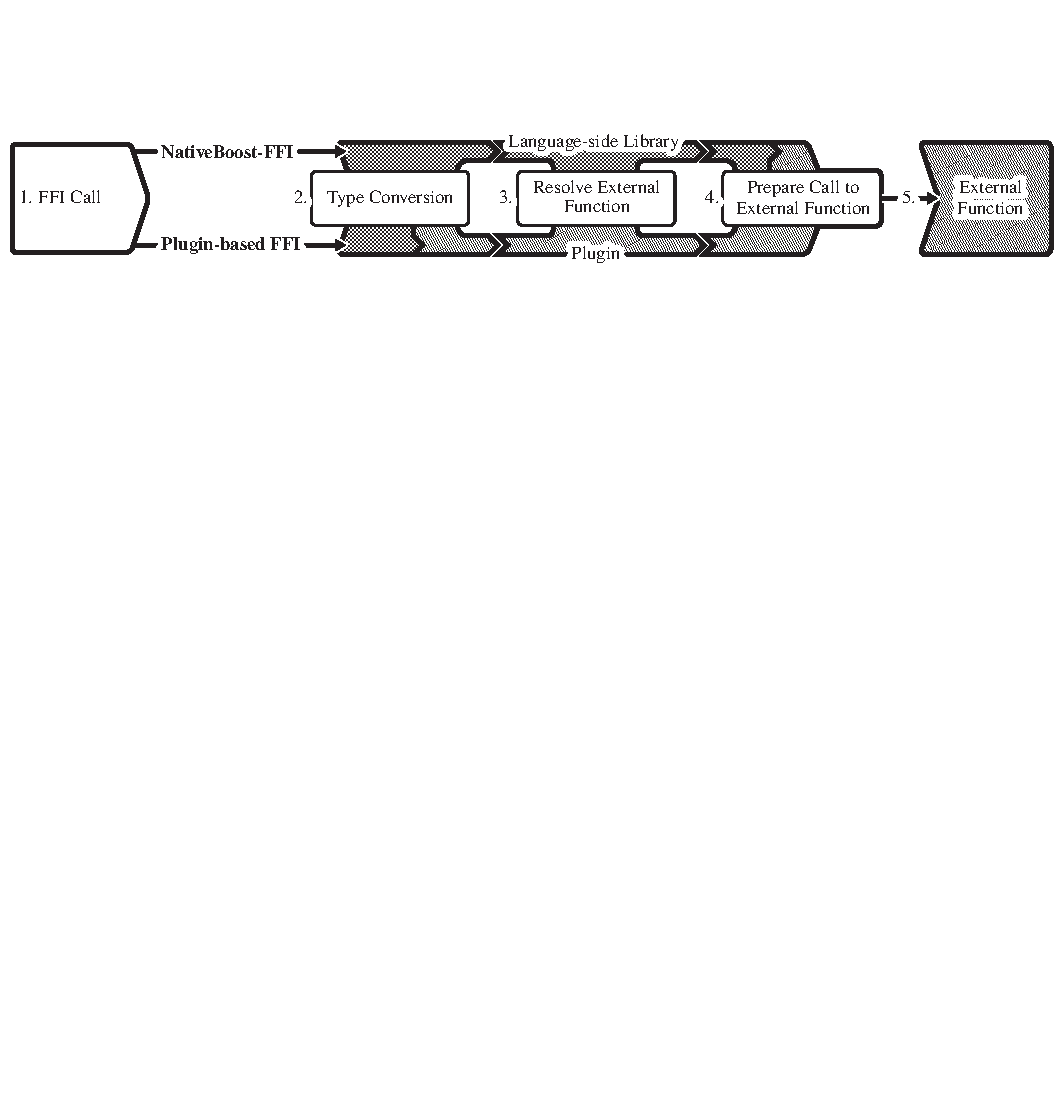
\includegraphics[scale=1.1]{ffiOverview}
	\end{adjustwidth}
	\caption[\FFI Implementation Comparison]{Comparison of \FFI calls propagation in \NBFFI and a typical \VM plugin-based implementation. \NB resorts to \VM-level only for the native-code activation, whereas typical implementations cross this barrier much earlier.}
	\figlabel{ffi-ffi}
\end{figure*}

% ===========================================================================
\section{\NBFFI Evaluation}
\seclabel{ffi-evaluation}
\seclabel{ffi-performance}
% ===========================================================================

In this section we compare \NB with other \FFI implementations.
\begin{description}
	\item[\Alien \FFI:] An \FFI implementation for \Squeak/\PH that focuses on the lan\-guage-side. All marshalling happens transparently at language-side.
	\item[C-\FFI:] A C based \FFI implementation for \Squeak/\PH that performs all marshalling operations at \VM-side.
	\item[\LuaJIT:] A fast \Lua implementation that has a close \FFI integration with \JIT interaction.
\end{description}

\paragraph{Choice of \FFI Implementations}
To evaluate \NB we explicitly target \FFI implementations running on the same platform, hence we can rule out additional performance differences.
\Alien and C-\FFI run in the same \PH image as \NB allowing a much closer comparison.
\Alien \FFI is implemented almost completely at language-side, much like \NB.
However, as the following benchmarks will stress, it also suffers from performance loss.
On the other end there is C-\FFI which is faster than \Alien but by far not as flexible.
For instance only primitive types are handled directly.
As the third implementation we chose \Lua which is widely used as scripting language in game development.
Hence much care has been taken to closely integrate \Lua into C and C++ environments.
\LuaJIT integrates an \FFI library that generates the native code for marshalling and directly inlines C functions callout in the \JIT-compiled code.

\paragraph{Evaluation Procedure}
To compare the different \FFI approaches we measure 100 times the accumulative time spent to perform $1'000'000$ callouts of the given function.
From the 100 probes we show the average and the standard deviation for a $68\%$ confidence interval in a gaussian distribution.
To exclude the calling and loop overhead we subtract from each evaluation the time spent in the same setup, but without the \FFI call.
The final deviation displayed is the arithmetic average of the measured deviation of the base and the callout measurement.

The three \FFI solutions that work in \PH (\NB, \Alien, C-\FFI) are evaluated on the very same \PH 1.4 (version 14458) image on a \PH \VM (version of May 5. 2013).
For the \Lua benchmarks we use \LuaJIT 2.0.1.
The benchmarks are performed under the constant conditions on a MacBook Pro.
Even though a standalone machine could improve the performance we are only interested in the relative performance of each implementation.


\paragraph{Choice of Callouts}
We chose a set of representative C functions to stress different aspects of an \FFI implementation.
We start with simple functions that require little marshalling efforts and thus mainly focus on the activation performance and callout overhead.
Later we measure more complex C functions that return complex types and thus stress the marshalling infrastructure.

% ---------------------------------------------------------------------------
\subsection{Callout Overhead}
% ---------------------------------------------------------------------------

The first set of \FFI callouts show mainly the overhead of the \FFI infrastructure to perform the callout.

For the first \FFI evaluation we measure the execution time for a \ttt{clock()} callout.
The C function takes no argument and returns an integer thus guaranteeing a minimal overhead for marshalling and performing the callout.
%
\begin{table}[H]
    \centering
    \begin{tabular}{rSS}
                     & {Call Time [ms]} & {Relative Time} \\\midrule
        \NB          & 492.13(73)       & 1.0 \\
        \Alien       & 606.6 (19)       & \approx 1.2\\
        C-\FFI       & 541.77(88)       & \approx 1.1\\
        \LuaJIT      & 343.0 (12)       & \approx 0.7
    \end{tabular}
    \caption{Speed comparison of an \ttt{uint clock(void)} \FFI call (see Code~\lstref{ffi-clock}).}
    \tablabel{ffi-performance-clock}
\end{table}
%
\noindent \ttt{abs} is a about the same complexity as the \ttt{clock} function, however accepting a single integer as argument.
%
\begin{table}[h!]
    \centering
    \begin{tabular}{rSS}
                & {Call Time [ms]} & {Relative Time} \\\midrule
        \NB     &  65.34(23)       &         1.00 \\
        \Alien  & 175.77(31)       & \approx 2.69 \\
        C-\FFI  & 148.77(21)       & \approx 2.27 \\
        \LuaJIT\tablefootnote{Downsampled from increased loop size by a factor $100$ to guarantee accuracy.}
                & 2.035(15)        & \approx 0.03
    \end{tabular}
    \caption{Speed comparison of an \ttt{int abs(int i)} \FFI call (see \figref{ffi-nativeBoostSyntax}).}
    \tablabel{ffi-performance-abs}
\end{table}


\paragraph{Evaluation}
For measuring the calling overhead we chose the \ttt{abs} \FFI callout.
This C function is completed in a couple of instructions which in comparison to the conversion and activation effort of the \FFI callout is negligible.
In \tabref{ffi-performance-abs} we see that \NB is at least a factor two faster than the other \PH implementation.
Yet \LuaJIT outperform \NB by an impressive factor 30.
\LuaJIT has a really close integration with the \JIT and this is what makes the impressive \FFI callout results possible.


% ---------------------------------------------------------------------------
\subsection{Marshalling Overhead for Primitive Types}
% ---------------------------------------------------------------------------

The third example calls \ttt{getenv('PWD')} expecting a string as result:  the path of the current working directory.
Both argument and result have to be converted from high-level strings to C-level zero-terminated strings.
%
\begin{table}[h!]
    \centering
    \begin{tabular}{rSS}
                    & {Call Time [ms]} & {Relative Time} \\\midrule
        \NB         &  105.29(24)      &          1.0 \\
        \Alien      & 1058.7 (20)      & \approx 10.1 \\
        C-\FFI      &  282.94(24)      & \approx  2.7 \\
        \LuaJIT\tablefootnote{Downsampled from increased loop size by a factor $10$ to guarantee accuracy.}
                    & 97.3(51)         & \approx 0.9
    \end{tabular}
    \caption{Speed comparison of an \ttt{char * getenv(char *name)} \FFI call (see Code \lstref{ffi-getenv}).}
    \tablabel{ffi-performance-getenv}
\end{table}

\noindent As a last evaluation of simple C functions with \NB, we call \ttt{printf} with a string and two integers as argument.
The marshalling overhead is less than for the previous \ttt{getenv} example.
However, \ttt{printf} is a more complex C function which requires more time to complete: it has to parse the format string, format the given arguments and pipe the results to standard out.
Hence the relative overhead of an \FFI call is reduced.
%
\begin{table}[h!]
    \centering
    \begin{tabular}{rSS}
                    & {Call Time [ms]}  & {Relative Time} \\\midrule
        \NB         &  371.03(51)       &         1.0 \\
        \Alien      & 1412.37(79)       & \approx 3.8 \\
        C-\FFI      &  605.02(23)       & \approx 1.6 \\
        \LuaJIT     &  202.4 (21)       & \approx 0.6
    \end{tabular}
    \caption{Speed comparison of an \ttt{int printf(char *name, int num1, int num2)} \FFI call}
    \tablabel{ffi-performance-printf}
\end{table}

\paragraph{Evaluation}
\tabref{ffi-performance-clock} and \tabref{ffi-performance-abs} call C functions that return integers for which the conversion overhead is comparably low.
However we see that \Alien compares worse in the case of more complex Strings.
\tabref{ffi-performance-getenv} and \tabref{ffi-performance-printf} show this behavior.
For the \ttt{getenv} a comparably long string is returned which causes a factor 10 conversion overhead for \Alien.


% ---------------------------------------------------------------------------
\subsection{Using Complex Structures}
% ---------------------------------------------------------------------------

To evaluate the impact of marshalling complex types, we measure the execution time for a callout to \ttt{cairo\_matrix\_multiply} described in \lstref{ffi-cairoCallouts}.
In all cases, the allocation time of the structs is not included in the measurement nor their field assignments.
\tabref{ffi-performance-structs} shows the results.

\begin{table}[h]
    \centering
    \begin{tabular}{rSS}
                    & {Call Time [ms]} & {Relative Time} \\\midrule
        \NB         &  79.00 (27)      &         1.0 \\
        \Alien      & 753.82 (51)      & \approx 9.5 \\
        C-\FFI      & 380.8  (27)      & \approx 3.6 \\
        \LuaJIT     &  5.66  (15)      & \approx 0.07
    \end{tabular}
    \caption{Speed comparison of an \ttt{cairo\_matrix\_multiply} \FFI call (cf. \lstref{ffi-cairoCallouts})}
 	\tablabel{ffi-performance-structs}
\end{table}

\paragraph{Evaluation}
\tabref{ffi-performance-structs} shows that \NB outperforms the two other \PH implementations.
\todo{moa text hea needed}

% ---------------------------------------------------------------------------
\subsection{Callbacks}
% ---------------------------------------------------------------------------

\tabref{ffi-performance-qsort} shows a comparison of \ttt{qsort} callouts passing callbacks.
Callbacks are usually much slower than callouts.

\begin{table}[h]
    \centering
    \begin{tabular}{rSS}
                    & {Call Time [ms]} & {Relative Time} \\\midrule
        \NB         & 2300.0 (11)      &         1.0 \\
        \Alien      &  600.83 (35)     & \approx 0.26 \\
        C-\FFI      & NA               & NA \\
        \LuaJIT     &   46.13(62)      & \approx 0.02\\ \cmidrule(r){2-3}
	\NB with Native Callbacks
	                & 4.98(21)  & \approx 0.002
    \end{tabular}
    \caption{Speed comparison of a \ttt{qsort} \FFI call (cf. \lstref{ffi-calloutWithCallback})}
 	\tablabel{ffi-performance-qsort}
\end{table}


\paragraph{Evaluation}
The results show that \NB callbacks are currently slower than \Alien's ones.
This is because \Alien relies on specific \VM support for callbacks making their activation faster (context creation and stack pages integration).
On the opposite, \NB currently uses small support from the \VM side and even do part of the work at image side.
This \ttt{qsort} demonstrates the worst case because it implies a lot of activations of the callback.
For each of these calls, \NB creates a context and make the \VM switch to it.
To really demonstrate that these context switches are the bottleneck, \tabref{ffi-performance-qsort} also shows the result of doing the same benchmark in \NB but using a native callback i.e. containing native code.
We do not argue here that callbacks should be implemented in native code but that \NB support for callback can be optimized to reach \Alien's performance at least.

% ===========================================================================
\section{\NBFFI Implementation Details}
\seclabel{ffi-internals}
% ===========================================================================

The following subsections will first focus on the high-level, language-side aspects of \NB, such as native code generation and marshalling.
As a second part we describe the low-level interaction of \NB with \B.

% ---------------------------------------------------------------------------
\subsection{Generating Native Code}
\seclabel{ffi-generating}
% ---------------------------------------------------------------------------

In \NB all code generation happens transparently at language-side.
The various examples shown in \secref{ffi-nutshell} show how an \FFI callout is defined in a standard method.
Upon first activation the \NB primitive will fail and by default continues to evaluate the following method body.
This is the point where \NB generates native code and attaches it to the compiled method.
\NB then reflectively resends the original message with the original arguments (for instance \ttt{abs:} in the example \figref{ffi-nativeBoostSyntax}).
On the second activation, the native code is present and thus the primitive will no fail but run the native code.
\secref{benzo-code-activation} will gave more internal details about the code activation and triggering of code generation.

% ---------------------------------------------------------------------------
\paragraph{Generating Assembler Instructions}

\figref{ffi-nbArchitecture} shows that \NB relies on \urlfootnote{AsmJit}{http://smalltalkhub.com/\#!/~Pharo/AsmJit/}, a language-side assembler.
AsmJit emerged from an existing \urlfootnote{C++ implementation}{http://code.google.com/p/asmjit/} and currently supports the x86 instruction set.
In fact it is even possible to inline custom assembler instructions in \PH when using \NB.
This way it is possible to meet critical performance requirements.
Typically \PH does not excel at algorithmic code since such code does not benefit from dynamic message sends.

% ---------------------------------------------------------------------------
\paragraph{Reflective Symbiosis}

\NB lives in symbiosis with the \PH programming environment.
As shown in the examples in \secref{ffi-nutshell} and in more detail in \figref{ffi-nativeBoostSyntax} \NB detects which method arguments correspond to which argument in the \FFI callout.
To achieve this, \NB inspects the activation context when generating native code.
Through reflective access to the execution context we can retrieve the method's source code and thus the argument names and positions.

% ---------------------------------------------------------------------------
\paragraph{Memory Management}
\NB supports external heap management with explicit allocation and freeing of memory regions.
There are interfaces for \ttt{allocate} and \ttt{free} as well as for \ttt{memcopy}:
%
\begin{stcode}[
	label={lst:ffi-externalHeap},
	caption={Example of external heap management in \NB}]{0}
memory := NativeBoost allocate: 4.
bytes  := #[1 2 3 4].
"Fill the external memory"
NativeBoost memCopy: bytes to: memory size: 4.

"FFI call to fill the external object"
self fillExternalMemory: memory.

"Copy back bytes from the external object"
NativeBoost memCopy: memory to: bytes size: 4.
NativeBoost free: memory.
\end{stcode}

\noindent Using the external heap management it is possible to prepare binary blobs and structures for \FFI calls.
In the previous example Code \lstref{ffi-externalHeap} the \ttt{memory} variable holds a wrapper for the static address of the allocated memory.
Hence accessing it from low-level code is straight forward.
However in certain situations it is required to access a high-level object from assembler.
\PH has a moving garbage collector which means that you can not refer directly to a high-level object by a fixed address.

As explained in more detail in \secref{benzo-gc-interaction} \B uses a special array at a known to deal with this problem.
Unlike normal \PH objects, this array has a known, fixed address that contains pointers to high-level objects.
The garbage collector keeps this external roots array up to date.
Hence it is possible to statically refer to a \PH object using a double indirection over the external roots.


% ---------------------------------------------------------------------------
\subsection{Activating Native Code}
% ---------------------------------------------------------------------------

In this section we present the \VM-level interaction of \NB.
Even though \NB handles most tasks directly at language-side it requires certain changes on \VM level:
%
\begin{itemize}[noitemsep]
	\item executable memory,
	\item activation primitives for native code.
\end{itemize}
%
Since \NB manages native code at language-side there is no special structure or memory region where native code is stored.
Native instructions are appended to compiled methods which reside on the heap.
Hence the heap has to be executable in order to jump to the native instructions.

\todo{small paragraph outlining the basic activation + link back to the benzo \secref{benzo-code-activation}}\\
\todo{\FFI-specific activation image}

% ===========================================================================
\section{Related Work}
\seclabel{ffi-relatedWork}
% ===========================================================================

Typical \ST system are isolated from the low-level world and provide only limited interoperability with C libraries.
However there are notable exceptions: \textsc{Étoilé} and \ST/X.

Chisnall presents the Pragmatic \ST Compiler \cite{Chis12a}, part of the \textsc{Étoilé} project, which focuses on close interaction with the C world.
The main goal of this work is to reuse existing libraries and thus reduce duplicated effort.
The author highlights the expressiveness of \ST to support this goal.
In this \ST implementation multiple languages can be mixed efficiently.
It is possible to mix Objective-C, \ST code.
All these operations can be performed dynamically at runtime.
Unlike our approach, \textsc{Étoilé} aims at a complete new style of runtime environment without a \VM.
Compared to that, \NB is a very lightweight solution.

Other dynamic high-level languages such as \Lua leverage \FFI performance by using a close interaction with the \JIT.
\urlfootnote{\LuaJIT}{https://github.com/jmckaskill/luaffi/} for instance is an efficient \Lua implementation that inlines \FFI calls directly into the \JIT compiled code.
Similar to \NB this allows one to minimize the constant overhead by generating custom-made native code.
The \LuaJIT runtime is mainly written in C which has clearly different semantics than \Lua itself.

On a more abstract level, high-level low-level programming \cite{Fram09a} encourage to use high-level languages for system programming.
Frampton et al. present a low-level framework  which is used as system interface for \Jikes, an experimental \Java \VM.
However their approach focuses on a static solution.
Methods have to be annotated to use low-level functionality.
Additionally the strong separation between low-level code and runtime does not allow for reflective extensions of the runtime.
Finally, they do not support the execution and not even generation of custom assembly code on the fly.

Kell and Irwin \cite{Kell11a} take a different look at interacting with external libraries.
They advocate a Python \VM that allows for dynamically shared objects with external libraries.
It uses the low-level \textsc{dwarf} debugging information present in the external libraries to gather enough metadata to automatically generate \FFIs.

% ===========================================================================
\section{Problems}
\seclabel{ffi-problems}
\seclabel{ffi-futurework}
% ===========================================================================

After presenting \NB with all its benefits in detail we also have to shed some light on its limitations in this section. 
The problems and limitations described in this section were discovered while using \NB extensively in \PH.
Since \NB is based on \B for the low-level programming part, most of \NB's limitations are the limitations of \B itself that were already presented previously in \secref{benzo-problems}.
In this section we will focus on the high-level problems and leave out the low-level limitations of \B as they are not the domain of \NB.
As such the major issue with \NB is the lack of a dedicated debugging infrastructure followed by a \NB-specific approach to support platform dependent code.

% ---------------------------------------------------------------------------
\subsection{Difficult Debug Cycles}
% ---------------------------------------------------------------------------
As a direct consequence from \B's shortcomings is the limited debugging support.
Once \NB generated the native code for the callout there is no possibility to interact with the code anymore.
We \B described in \secref{benzo-problems-robustness} that there is not special debugging mode available and native code is run unprotected.
As a result, errors happening inside external libraries have fatal consequences in \NB: the process running the \PH image is terminated.
The core of this problem has to be addressed at \B-level and not directly in \NB.

In a future version of \NB, together with improvements of the underlying \B debugging infrastructure (see \secref{benzo-problems-debugging}), we envision a seamless interaction with the external libraries.
There should be no barrier between \PH and external code, a more sophisticated debugger could dynamically switch context and start displaying more C oriented information in the external library.
In the worst case we could still display native instructions and inspect the stack as we step through the external function.
In best case we could provide a \GDB-like debugging experience with source code and resolved symbol names.

% ---------------------------------------------------------------------------
\subsection{Platform Independence}
% ---------------------------------------------------------------------------
The second problem we would like to address is platform independence.
This is certainly a crucial issue for any framework that deals with native code and as such a main concern of \B (see \secref{benzo-problems-platform-independence}).
However, the instruction-level architecture support is of secondary importance for \NB as it interacts mostly on operating system level.
Rewriting \NB's explicit assembler routines in the platform independent intermediate representation (\VCPU) presented in \secref{benzo-problems-vcpu} would solve the \CPU architecture dependency.

Currently \NB is used on three operating system: \Linux, \textsc{Mac OS X} and \Windows.
Internally \NB already deals with different calling conventions C-functions on the different platforms.
Nevertheless, from a user point of view it is mandatory to have a well defined way to deal with platform specific \FFI callouts.
The current approach as outlined for the \PH \OS environment variables object in \secref{reification-simple} is to create a specific subclass for each platform.
A simple extension to \NB to allow callout definitions for multiple platforms in a single method would greatly improve this case.
The following code example illustrates a possible solution:
%
\begin{stcode}[]{}
FFI 
  unix: [ :builder |
    builder 
      nbCall: #(int setenv(
                      String name, String value, 1 ))
      module: NativeBoost CLibrary ];
  windows: [ :builder |
    builder
      nbCall: #(int SetEnvironmentVariableA(
                      String name, String value ))
      module: #Kernel32
      options: #(optStringOrNull) ].
\end{stcode}
%
This examples includes the platform specific version for accessing an environment variable.
In this case the difference of the two platforms is handled by simply using a different native function.
However, already in the case of \ttt{getenv} function, \Windows and \unix implementations behave fundamentally different from \Windows' \ttt{GetEnvironmentVariableA} and a small \PH helper method is necessary to overcome the differences.
In this case it would be nice to mix \PH code and \FFI callouts more vividly and for instance allow inline \PH code in the example above.

% ---------------------------------------------------------------------------
\subsection{Limited Expressiveness}
% ---------------------------------------------------------------------------

\NB has been designed to call a single external function per callout.
To our knowledge this is the standard in \FFI implementations.
For most of the use cases this is sufficient but during development we found a peculiar case, when using \ttt{fork}, where two C function consecutive calls have to be made.
\ttt{fork} creates a new process at \OS-level.
It returns $0$ in the newly forked process and the new process id to the original parent process.
Hence a typical \ttt{fork} usage in C looks as follows:
%
\begin{ccode}{}
pid_t pid;
int status = 0;
// spawn child process 
if(!(pid = fork())) {
	// execute code in the child process
	....
	// stop the child process
	exit(EXIT_SUCCESS);
}
// in the parent process wait for the child process
waitpid(pid, &status, 0);	
\end{ccode}
%
Currently it is not possible to express this directly in \NB due to the \VM.
Imagine the following hypothetical \NB-based implementation of the previous example:
%
\begin{stcode}{}
pid := FFI fork.
pid isZero
	ifTrue: [ 
		self childProcessMethod.
		FFI exit: 0 ]
	ifFalse: [ 
		FFI waitPid: pid for: 10 seconds ]
\end{stcode}
%
The first two lines pose a significant problem, still ignoring the implementation details of the rest of the method.
What happens when we call \ttt{fork} with an \FFI callout?
Essentially this creates a fork of the whole \VM running \PH which has some side-effects since the resources between the child and the parent \VM process are shared.
\todo{maybe present the full details...}
In consequence when the \FFI callout for \ttt{fork} finishes, the \VM continues interpreting \PH code which in some cases stops to work due to the aforementioned side-effects.
This could technically be avoided if the solve purpose of the child process is to execute some native code in the background and the exit.
One would have to make sure that the sequence, \ttt{fork}, \textsc{pid} check, \ttt{exit} happens all in native code without handing over execution to \PH in between.
Which brings us back to the original observation that we cannot create a combined \FFI callout for multiple methods in \NB.

To solve this we could allow \NB to mix assembler instructions (or the more abstract \VCPU instructions) with multiple callouts.
Currently this almost possible by manually invoking the callout generator for different C functions.
However, there are certain side-effects with the stack-management which require more work.


% ---------------------------------------------------------------------------
\subsection{Startup Recursion}
\seclabel{ffi-startup-recursion}
% ---------------------------------------------------------------------------

Starting with \PH 3.0 we tried to slowly replace \VM plugin functionality with direct \FFI callouts at language-side.
This is an attempt to make language more open and shift a part of the development done in C at \VM-level to \PH.
The driving motivation is the same as for \NB itself: accessible and flexible code.

The \OS environment implementation based on \NB described earlier in \secref{reification-simple} was such an attempt.
In return it allowed us to add functionality to access to known directory locations under \Linux by directly or indirectly querying environment variables such as \ttt{HOME}.
In a second refactoring the functionality for opening the changes-file in \PH containing the changelog was made more flexible supporting more file locations.
This last change introduced a recursive dependency that is not visible on the first sight and illustrated in the following figure.
%
\begin{figure}[h]
	\centering
	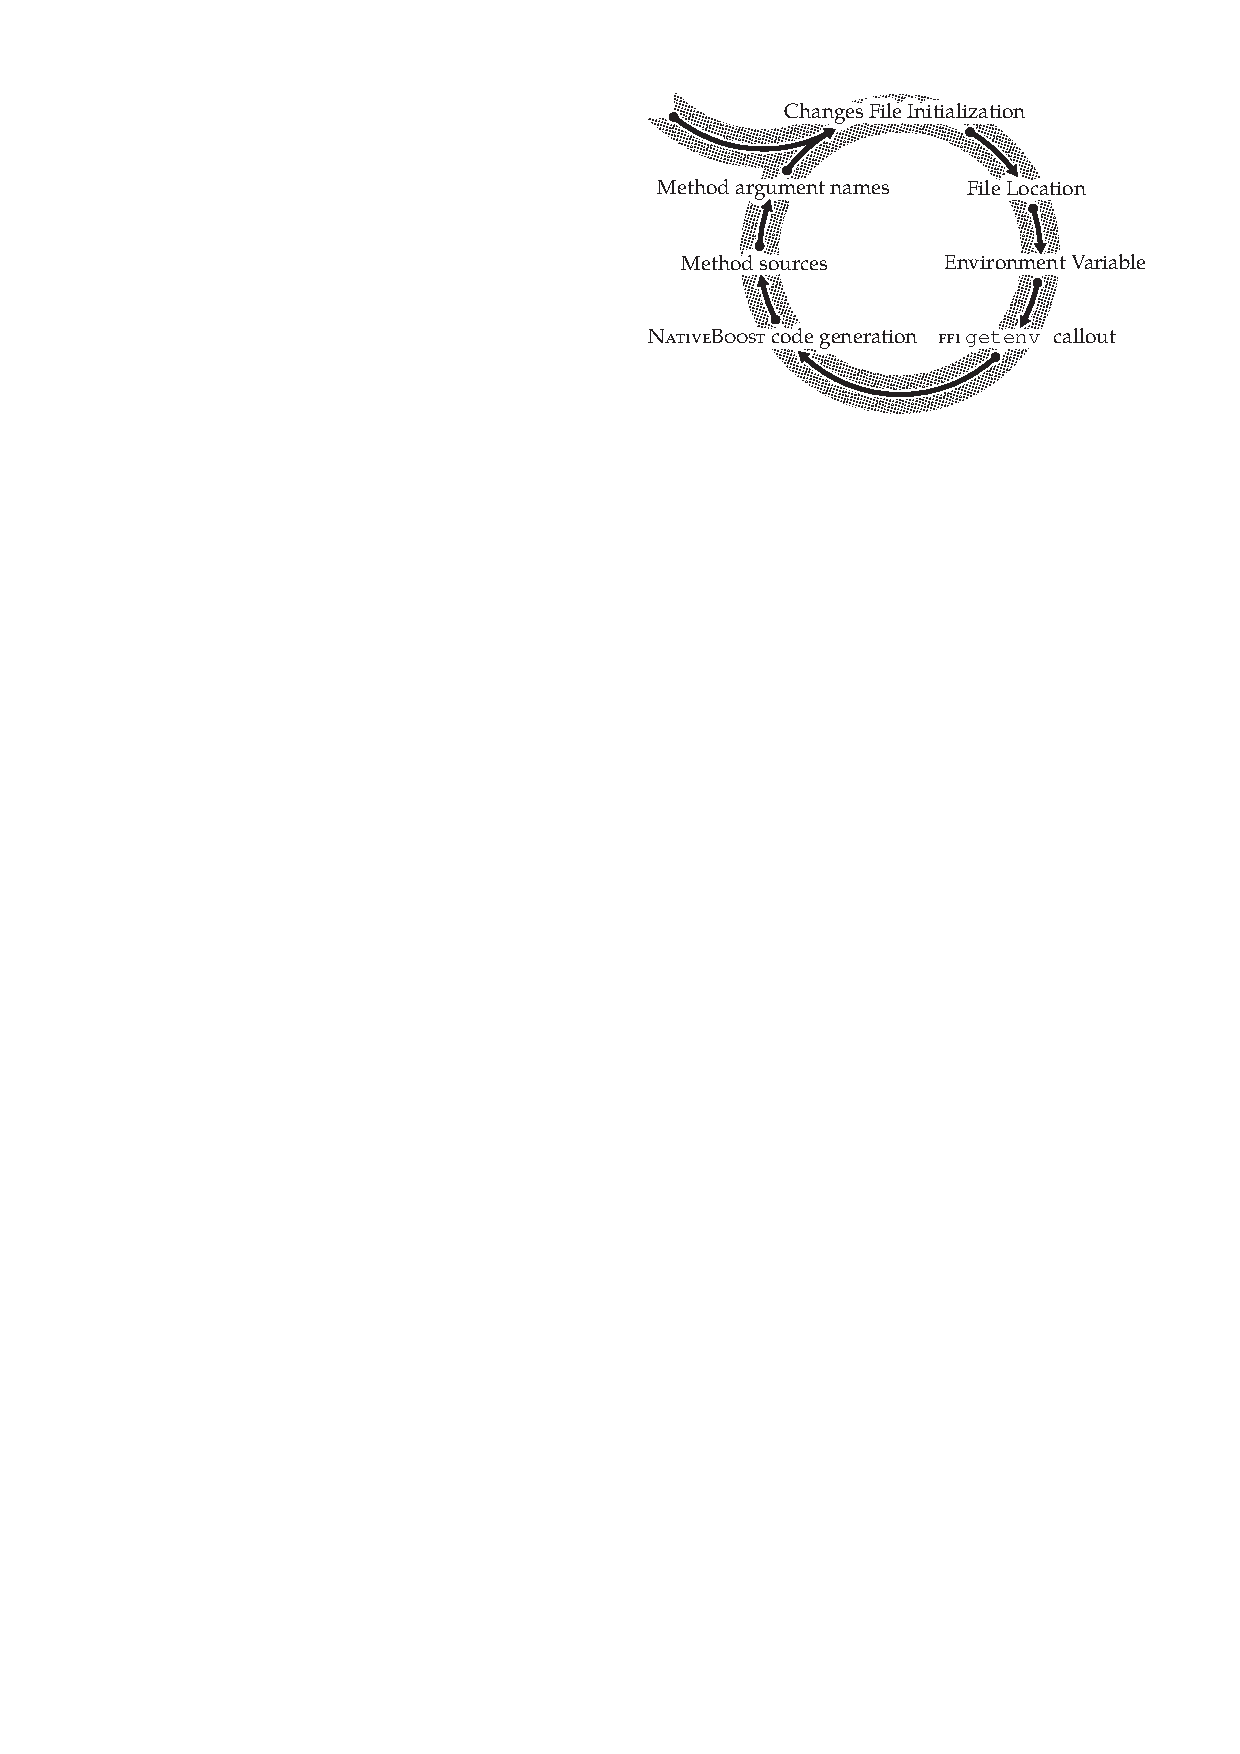
\includegraphics[scale=1.1]{nb-bootstrap-cycle}
\end{figure}
%
Essentially this meant that in certain cases where \NB required to compile the native code for callout it was impossible to start up \PH.
Once the native code was cached this recursion chain was broken and subsequently \PH started up well.

This particular issue was solved in \PH by caching the argument names in \NB used for assigning the \PH arguments to the callout parameters (see \secref{ffi-callout-parameters}).
The downside of this approach is that \NB reimplements part of \PH's existing reflection.
Of course there are other possibilities to avoid the described situation: deferred startup logics, lazy startup or storing the complete \PH source code in the image.
However, they would leave the general problem of using \NB during startup which might happen more often if more \VM plugins are replaced with \FFI callouts.
And even more general, how do we enable \NB on a system that does not allow dynamic code generation?
The only solution to this problem is to generate the \FFI callouts upfront and make these binaries available to the final product.
\todo{somehow missing ending}

% ---------------------------------------------------------------------------
\subsection{Performance}
% ---------------------------------------------------------------------------
Even though \NB shows good overall performance when it comes to callbacks it does not keep up with other \ST-based solutions.
In the current development phase not much attention was payed to callback performance as it is not a common use case for \FFI callouts.
Fast callbacks require close interaction and specific modifications at \VM-level.
However, initially \NB kept the modifications to the \VM at a minimum.
We assume that we can reach the same performance as \Alien relying on the same low-level implementation.

As a second issue we would like to address the callout overhead by using an already existing \JIT integration of \NB.
Currently the \VM has to leave from \JIT-mode to standard interpretation mode when it activates an \NB method.
This context switch introduces an unnecessary overhead for an \FFI callout.
A current prototype directly inlines the native code of a \NB method in the \JIT.
Hence the cost for the context switch plus the cost of activating the \NB callout primitive can be avoided.


% ===========================================================================
\section{Conclusion}
\seclabel{ffi-conclusion}
% ===========================================================================
\todo{make proper summary and mention more \B}
In this chapter we presented \NB a novel approach to foreign function interfaces.
Our approach relies only on a very generic extension of the \VM to allow for language-side code to directly call native instructions.

Using a in depth evaluation of \NB comparing against two other \ST \FFI implementations and \LuaJIT we showed in \secref{ffi-evaluation} that our language-side approach is competitive.
\NB reduces the callout overhead by more than a factor two compared to the two closest \ST solutions.

Compared to \LuaJIT there is still space for improvements.
We measured a factor 30 lower calling overhead due to a close \JIT integration.
However for typical \FFI calls the absolute time difference between \NB and \Lua is roughly $30\%$.
With a partial solution ready to integrate \NB closer with the \JIT we expect to come close to \Lua's performance.

Furthermore we showed that \NB essentially combines \VM-level performance with language-side flexibility when it comes to marshal complex types.
New structures are defined practically at language-side and conversion optimizations are added transparently.

% =============================================================================
\ifx\wholebook\relax\else
    \end{document}
\fi
